%%%%%%%%%%%%%%%%%%%%%%%%%%%%%%%%%%%%%%%%%%%%%%%%%%%%%%%%%%%%%%%%%%%%%%%%%%%%%%%
\documentclass[hyperref={pdfpagelabels=false},compress,table]{beamer} % 在Mac下无法编译
% \documentclass[compress,table]{beamer} % 在Mac下使用
% package for font
\usepackage{fontspec}
\defaultfontfeatures{Mapping=tex-text}  %%如果没有它,会有一些 tex 特殊字符无法正常使用,比如连字符。
\usepackage{xunicode,xltxtra}
\usepackage[BoldFont,SlantFont,CJKnumber,CJKchecksingle]{xeCJK}  % \CJKnumber{12345}: 一万二千三百四十五
\usepackage{CJKfntef}  %%实现对汉字加点、下划线等。
\usepackage{pifont}  % \ding{}
% package for math
\usepackage{amsfonts}

% package for graphics
\usepackage[americaninductors,europeanresistors]{circuitikz}
\usepackage{tikz}
\usetikzlibrary{plotmarks}  % placements=positioning
\usepackage{graphicx}  % \includegraphics[]{}
\usepackage{subfigure}  %%图形或表格并排排列
% package for table
\usepackage{colortbl,dcolumn}  %% 彩色表格
\usepackage{multirow}
\usepackage{multicol}
\usepackage{booktabs}
% package for code
\usepackage{fancyvrb}
\usepackage{listings}

% \usepackage{animate}
% \usepackage{movie15}

%%%%%
% setting for beamer
\usetheme{default} % Madrid(常用), Copenhagen, AnnArbor, boxes(白色), Frankfurt,Berkeley
\useoutertheme[subsection=true]{miniframes} % 使用Berkeley时注释本行
\usecolortheme{sidebartab}
\usefonttheme{serif}  %%英文使用衬线字体
% \setbeamertemplate{background canvas}[vertical
% shading][bottom=white,top=structure.fg!7] %%背景色,上25%的蓝,过渡到下白。
\setbeamertemplate{theorems}[numbered]
\setbeamertemplate{navigation symbols}{}  %% 去掉页面下方默认的导航条
\setbeamercovered{transparent}  %设置 beamer 覆盖效果

% 设置标题title背景色
% \setbeamercolor{title}{fg=black, bg=lightgray!60!white}
\setbeamercolor{title}{fg=white, bg=black!70!white}

% 设置每页小LOGO
\pgfdeclareimage[width=1cm]{ouc}{figures/static/ouc.pdf}
\logo{\pgfuseimage{ouc}{\vspace{-20pt}}}

% setting for font
%%\setCJKmainfont{Adobe Kaiti Std}
\setCJKmainfont{SimSun} 
%% \setCJKmainfont{FangSong_GB2312} 
%% \setmainfont{Apple Garamond}  %%苹果字体没有SmallCaps
\setCJKmainfont{SimSun} 
%FUNNY%\setCJKmainfont{DFPShaoNvW5-GB}  %%华康少女文字W5(P)
%FUNNY%\setCJKmainfont{FZJingLeiS-R-GB}  %%方正静蕾体
%FUNNY%\setmainfont{Purisa}
%\setsansfont[Mapping=tex-text]{Adobe Song Std}
     %如果装了Adobe Acrobat,可在font.conf中配置Adobe字体的路径以使用其中文字体。
     %也可直接使用系统中的中文字体如SimSun、SimHei、微软雅黑等。
     %原来beamer用的字体是sans family;注意Mapping的大小写,不能写错。
     %设置字体时也可以直接用字体名,以下三种方式等同:
     %\setromanfont[BoldFont={黑体}]{宋体}
     %\setromanfont[BoldFont={SimHei}]{SimSun}
     %\setromanfont[BoldFont={"[simhei.ttf]"}]{"[simsun.ttc]"}
% setting for graphics
\graphicspath{{figures/}}  %%图片路径
\renewcommand\figurename{图}

% setting for pdf
\hypersetup{% pdfpagemode=FullScreen,%
            pdfauthor={Xiaodong Wang},%
            pdftitle={Title},%
            CJKbookmarks=true,%
            bookmarksnumbered=true,%
            bookmarksopen=false,%
            plainpages=false,%
            colorlinks=true,%
            citecolor=green,%
            filecolor=magenta,%
            linkcolor=blue,%red(default)
            urlcolor=cyan}

% setting for fontspec
\XeTeXlinebreaklocale "zh"  %%表示用中文的断行
\XeTeXlinebreakskip = 0pt plus 1pt minus 0.1pt  %%多一点调整的空间
%%%%%

% font setting by xeCJK
\setCJKfamilyfont{NSimSun}{NSimSun}
\newcommand{\song}{\CJKfamily{NSimSun}}
%%%\setCJKfamilyfont{AdobeSongStd}{Adobe Song Std}
%%%\newcommand{\AdobeSong}{\CJKfamily{AdobeSongStd}}
\setCJKfamilyfont{FangSong}{FangSong_GB2312}
\newcommand{\fang}{\CJKfamily{FangSong}}
%%%\setCJKfamilyfont{AdobeFangsongStd}{Adobe Fangsong Std}
%%%\newcommand{\AdobeFang}{\CJKfamily{AdobeFangsongStd}}
\setCJKfamilyfont{SimHei}{SimHei}
\newcommand{\hei}{\CJKfamily{SimHei}}
%%%\setCJKfamilyfont{AdobeHeitiStd}{Adobe Heiti Std}
%%%\newcommand{\AdobeHei}{\CJKfamily{AdobeHeitiStd}}
\setCJKfamilyfont{KaiTi}{KaiTi}
\newcommand{\kai}{\CJKfamily{KaiTi}}
%%%\setCJKfamilyfont{AdobeKaitiStd}{Adobe Kaiti Std}
\newcommand{\AdobeKai}{\CJKfamily{AdobeKaitiStd}}
\setCJKfamilyfont{LiSu}{LiSu}
\newcommand{\li}{\CJKfamily{LiSu}}
\setCJKfamilyfont{YouYuan}{YouYuan}
\newcommand{\you}{\CJKfamily{YouYuan}}
\setCJKfamilyfont{FZJingLei}{FZJingLeiS-R-GB}
\newcommand{\jinglei}{\CJKfamily{FZJingLei}}
\setCJKfamilyfont{MSYH}{Microsoft YaHei}
\newcommand{\msyh}{\CJKfamily{MSYH}}

% 自定义颜色
\def\Red{\color{red}}
\def\Green{\color{green}}
\def\Blue{\color{blue}}
\def\Mage{\color{magenta}}
\def\Cyan{\color{cyan}}
\def\Brown{\color{brown}}
\def\White{\color{white}}
\def\Black{\color{black}}

\lstnewenvironment{xmlCode}[1][]{% for Java
  \lstset{
    basicstyle=\tiny\ttfamily,%
    columns=flexible,%
    framexleftmargin=.7mm, %
    % frame=shadowbox,%
    % rulesepcolor=\color{cyan},%
     frame=single,%
    backgroundcolor=\color{white},%
    xleftmargin=4\fboxsep,%
    xrightmargin=4\fboxsep,%
    numbers=left,numberstyle=\tiny,%
    numberblanklines=false,numbersep=7pt,%
    language=xml, %
    }\lstset{#1}}{}

\lstnewenvironment{javaCode}[1][]{% for Java
  \lstset{
    basicstyle=\tiny\ttfamily,%
    columns=flexible,%
    framexleftmargin=.7mm, %
    frame=shadowbox,%
    rulesepcolor=\color{cyan},%
    % frame=single,%
    backgroundcolor=\color{white},%
    xleftmargin=4\fboxsep,%
    xrightmargin=4\fboxsep,%
    numbers=left,numberstyle=\tiny,%
    numberblanklines=false,numbersep=7pt,%
    language=Java, %
    }\lstset{#1}}{}

\lstnewenvironment{shCode}[1][]{% for Java
  \lstset{
    basicstyle=\scriptsize\ttfamily,%
    columns=flexible,%
    framexleftmargin=.7mm, %
    frame=shadowbox,%
    rulesepcolor=\color{brown},%
    % frame=single,%
    backgroundcolor=\color{white},%
    xleftmargin=4\fboxsep,%
    xrightmargin=4\fboxsep,%
    numbers=left,numberstyle=\tiny,%
    numberblanklines=false,numbersep=7pt,%
    language=sh, %
    }\lstset{#1}}{}

\newcommand\ask[1]{\vskip 4bp \tikz \node[rectangle,rounded corners,minimum size=6mm,
  fill=white,]{\Cyan \includegraphics[height=1.5cm]{question} \Large \msyh #1};}

\newcommand\wxd[1]{\vskip 4bp \tikz \node[rectangle,minimum size=6mm,
  fill=blue!60!white,]{\White \ding{118} \msyh #1};}

\newcommand\xyy[1]{\vskip 2bp \tikz \node[rectangle,minimum size=3mm,
  fill=black!80!white,]{\White \msyh\scriptsize #1};}

\newcommand\cxf[1]{\vskip 4bp \tikz \node[rectangle,rounded corners,minimum size=6mm,
  fill=orange!60!white,]{\White \ding{42} \msyh #1};}

\newcommand\samp[1]{\vskip 2bp \tikz \node[rectangle,minimum size=3mm,
  fill=white!100!white,]{\Mage\msyh \small CODE \ding{231} \Black #1};\vskip -8bp}

\newcommand\zhyfly[1]{\tikz \node[rectangle,rounded corners,minimum size=6mm,ball color=red!25!blue,text=white,]{#1};}

\setbeamerfont{frametitle}{series=\msyh} % 修改Beamer标题字体

\makeatletter
\newcommand{\Extend}[5]{\ext@arrow 0099{\arrowfill@#1#2#3}{#4}{#5}}
\makeatother


%%%%%%%%%%%%%%%%%%%%%%%%%%%%%%%%%%%%%%%%%%%%%%%%%%%%%%%%%%%%%%%%%%%%%%%%%%%%%%%
% \titlepage
\title[KevinW@OUC]{\hei {\huge Java EE企业应用系统设计}\\  
 Java EE体系结构}
\author[王晓东]{王晓东\\
  \href{mailto:wangxiaodong@ouc.edu.cn}{\footnotesize wangxiaodong@ouc.edu.cn}}
\institute[中国海洋大学]{\small 计算机科学与技术系}
\date{\today}
\titlegraphic{\vspace{-6em}
\includegraphics[height=6cm]{static/ouc.pdf}\vspace{-6em}}
%%%%%%%%%%%%%%%%%%%%%%%%%%%%%%%%%%%%%%%%%%%%%%%%%%%%%%%%%%%%%%%%%%%%%%%%%%%%%%%
\begin{document}
%% Delete this, if you do not want the table of contents to pop up at
%% the beginning of each subsection:
\AtBeginSection[]{                              % 在每个Section前都会加入的Frame
  \frame<handout:0>{
    \frametitle{\textbf{\hei 接下来…}}
    \tableofcontents[currentsection]
  }
}  %

\AtBeginSubsection[]                            % 在每个子段落之前
{
  \frame<handout:0>                             % handout:0 表示只在手稿中出现
  {
    \frametitle{\textit{\hei 接下来…}}\small
    \tableofcontents[current,currentsubsection] % 显示在目录中加亮的当前章节
  }
}
 \frame{\titlepage}

%%%%%%%%%%%%%%%%%%%%%%%%%%%%%%%%%%%%%%%%%%%%%%%%
\begin{frame}
\frametitle{参考书目}
\begin{enumerate}
\item 吕海东,张坤 编著,Java EE企业级应用开发实例教程,清华大学出版社,2010年8月
\end{enumerate}  
\end{frame}

% \begin{frame}
% \frametitle{本章学习目标}
% \begin{enumerate}
% \item 
% \end{enumerate}  
% \end{frame}

\section*{大纲}
\frame{\frametitle{大纲} \tableofcontents }

\section{软件开发现状和发展趋势}
\begin{frame}[fragile] % [fragile]参数使得能够插入代码
\frametitle{软件开发现状}

\begin{description}
\item[\fbox{面向Internet}] 开发企业级Web应用
\item[\fbox{面向对象}] OOA/OOD/OOP,Java、C\#
\item[\fbox{面向组件}] 软件系统是由许多小的组件构建和装配起来的
\item[\fbox{采用标准规范开发}] J2EE, MS.NET
\item[\fbox{全面采用框架技术}] Struts、Spring、Hibernate、AJAX、WebWork
\item[\fbox{软件系统采用分层结构和设计模式}] MVC
\item[\fbox{工厂化流水线开发模式}] CVS
\item[\fbox{可视化软件建模}] UML、RUP、ROSE
\end{description}
\end{frame}

\section{Java EE概述}

\begin{frame}
\frametitle{Java EE定义} 

Java EE是基于Java SE标准版基础上的一组开发以服务器为中心的企业级应用的相关技术和规范,用
于规范化、标准化以Java为开发语言的企业级软件的开发、部署和管理,以减少开发费用、软件复杂
性和快速交付的目的。

\begin{figure}
\centering
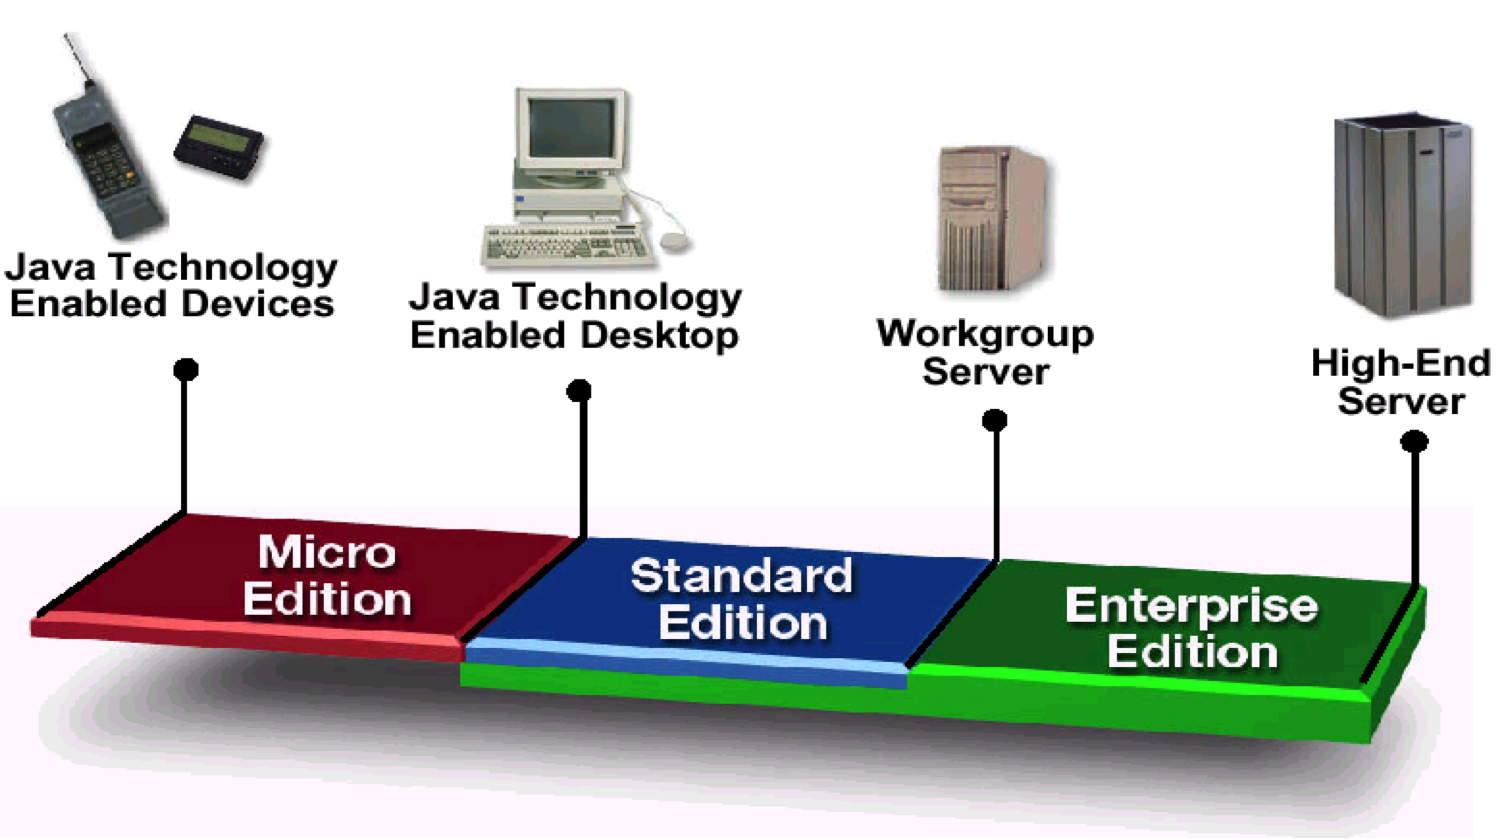
\includegraphics[width=0.7\textwidth]{fig01.png}
\end{figure}
\end{frame}

\begin{frame}
\frametitle{Java EE平台的总体结构} 
\begin{figure}
\centering
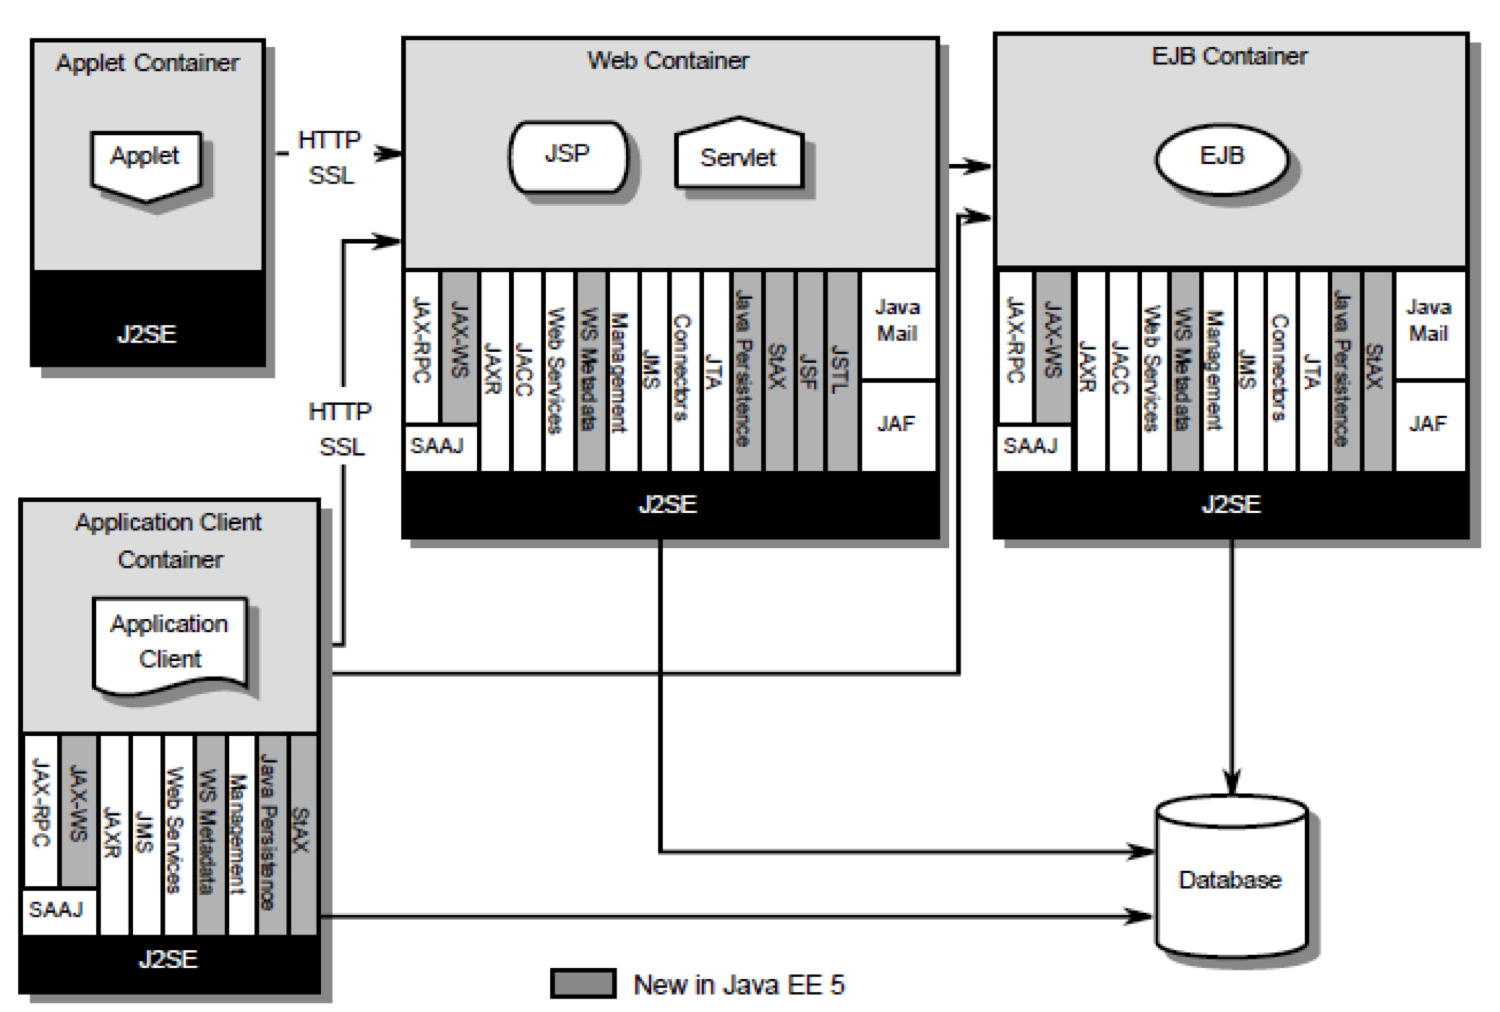
\includegraphics[width=0.85\textwidth]{fig02.png}
\end{figure}
\end{frame}

\begin{frame}
\frametitle{Java EE规范} 

Java EE规范定义了面向Internet的企业级软件应用的组成部分和各组成部分之间的交互协议。

\begin{itemize}[<+-| alert@+>]\kai
\item 容器规范\\
\only<1>{容器(Container)是组件的运行环境,负责组件的生命周期管理和调用。}
\item 组件规范\\
\only<2>{组件(Component)是Java EE应用的标准化部件,完成系统的业务和逻辑功能,在Java EE应用中组件运行在容器内,由容器管理组件的创建、调用和销毁整个生命周期。在Java EE应用中组件之间是不能直接调用的,必须通过容器完成。}
\item 服务规范\\
\only<3>{Java EE规定了连接各种外部资源的标准接口API,简化了连接各种不同类型外部资源的设计和编程。如JDBC API提供了连接数据库的标准接口;JMS API可以连接各种外部的消息服务系统。}
\item 通信协议规范\\
\only<4>{Java EE规范使用目前市场上主流的通信协议HTTP、HTTPS等,改进了与其他平台的互操作性。}
\item 开发角色规范\\
\only<5>{Java EE分别定义了7种不同的角色合作进行应用系统的开发,确保系统开发高效而有序,提高软件的成功率。}
\end{itemize}
\end{frame}

\section{Java EE容器}

\begin{frame}
\frametitle{Java EE容器(Container)} 

\begin{block}{容器}
容器是运行组件的环境对象,提供了组件运行所需要的服务,并管理组件的生成、调用和销毁整个生命周期。在Java EE规范下,所有Java EE组件都由容器来创建和销毁。
\end{block}
\begin{itemize}
\item 简化了企业级软件开发中复杂的对象管理事务
\item 克服了C++语言等内存泄漏缺陷
\end{itemize}
\end{frame}

\begin{frame}
\frametitle{Java EE容器类型} 
\begin{figure}
\centering
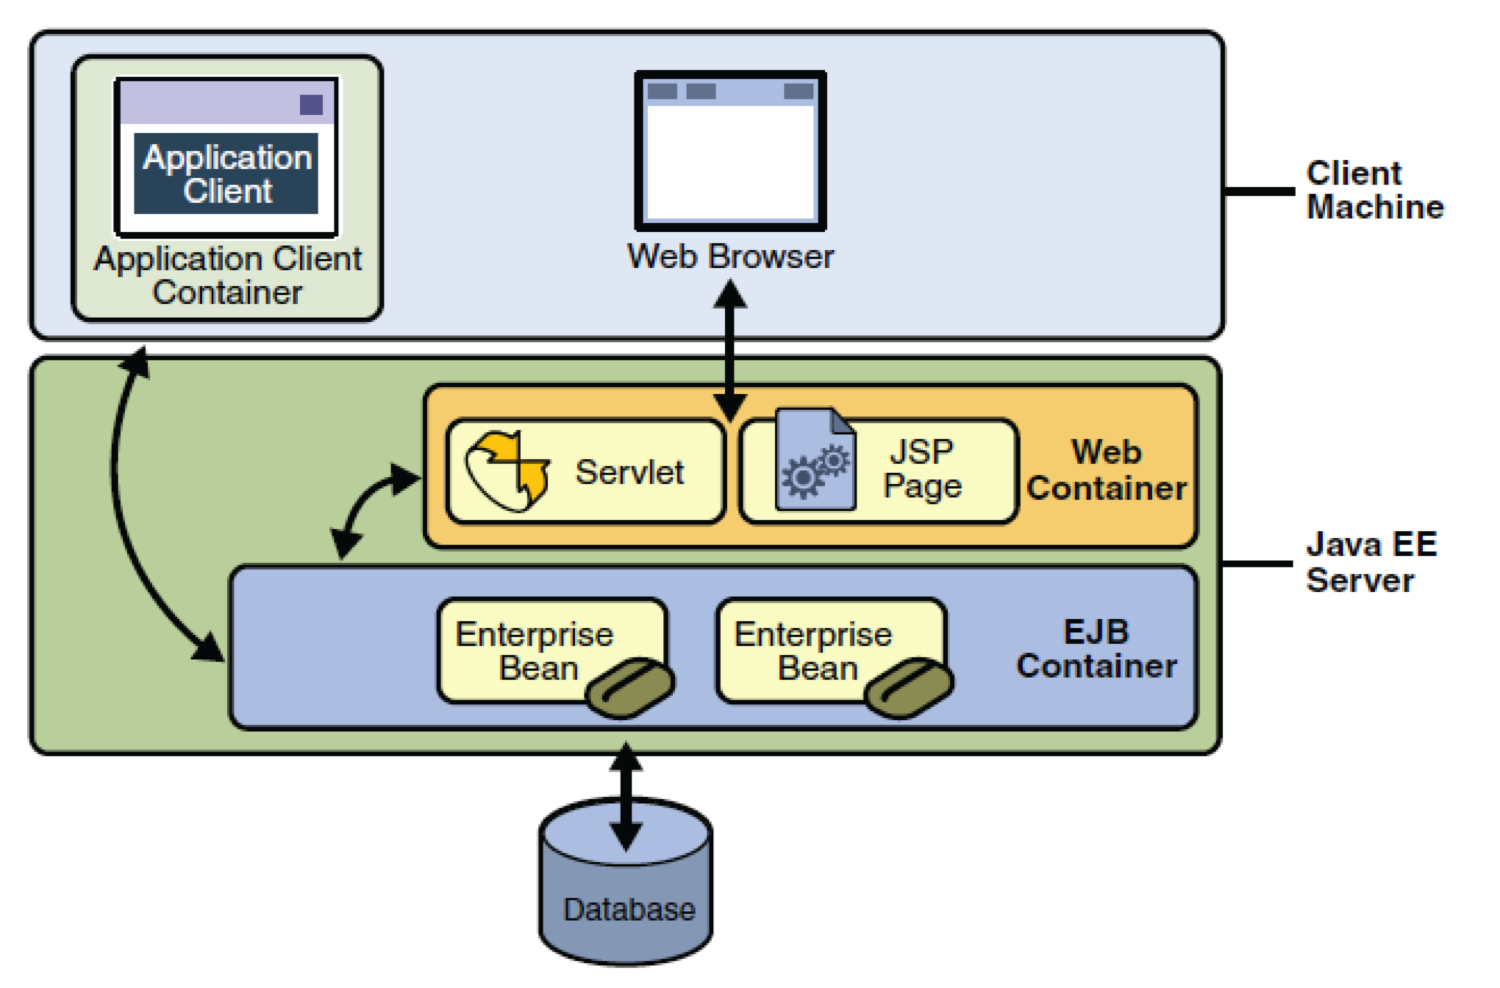
\includegraphics[width=0.85\textwidth]{fig04.png}
\end{figure}
\end{frame}

\begin{frame}
\frametitle{客户端应用容器} 

\begin{itemize}
\item 客户端应用容器(Application Client Container)即是普通Java SE的JVM,管理和运行客户JavaBean组件,与一般的Java类没有区别。
\item Java EE规范只是将它纳入自己的管理范围之内,进行统一的约定。
\item 客户端应用容器只能运行JavaBean组件。
\end{itemize}
\end{frame}

\begin{frame}
\frametitle{Applet容器} 
\begin{itemize}
\item Applet容器(Applet Container)是具有Java SE Plugin插件的Web浏览器,驻留在客户端,管理和运行Java Applet组件。
\item Applet容器使得Web具有丰富的图形界面和事件响应机制,进而开发出具有极高交互性的Web应用软件。
\end{itemize}
\end{frame}

\begin{frame}
\frametitle{Web容器} 
\begin{itemize}
\item Web容器(Web Container)管理Web组件的运行和调用。Java EE定义了两种Web组件:Servlet和JSP,可以产生动态Web内容,结合数据库技术,用于动态Web应用的开发。
\item Web容器运行在符合Java EE规范的应用服务器上,驻留在服务器端,外部应用可以通过HTTP和HTTPS协议与Web容器通信,进而访问Web容器管理的Web组件。
\end{itemize}
\end{frame}

\begin{frame}
\frametitle{企业JavaBean容器} 
\begin{itemize}
\item EJB容器(EJB Container)用于管理企业级JavaBean对象的生命周期和方法调用。Java EE规范定义了3种运行在EJB容器内的组件:{\hei 会话EJB、消息驱动EJB和实体EJB},分别完成不同领域的业务处理。
\item EJB容器运行在符合Java EE的应用服务器内,驻留在服务器端。
\item 其他组件通过RMI/IIOP协议与EJB容器通信,通过EJB容器来访问EJB组件的业务方法。
\end{itemize}
\end{frame}

\section{Java EE组件}
\begin{frame}
\frametitle{Java EE组件(Component)} 

\begin{itemize}
\item Java EE规范约定组成企业级软件系统的组成单元是组件。
\item 组件符合特定Java EE规范,对外发布服务接口。
\item 组件使用特定的配置信息部署在符合Java EE规范的服务器上运行,并与其他组建组装在一起,组成整个Java EE应用系统。
\end{itemize}
\begin{figure}
\centering
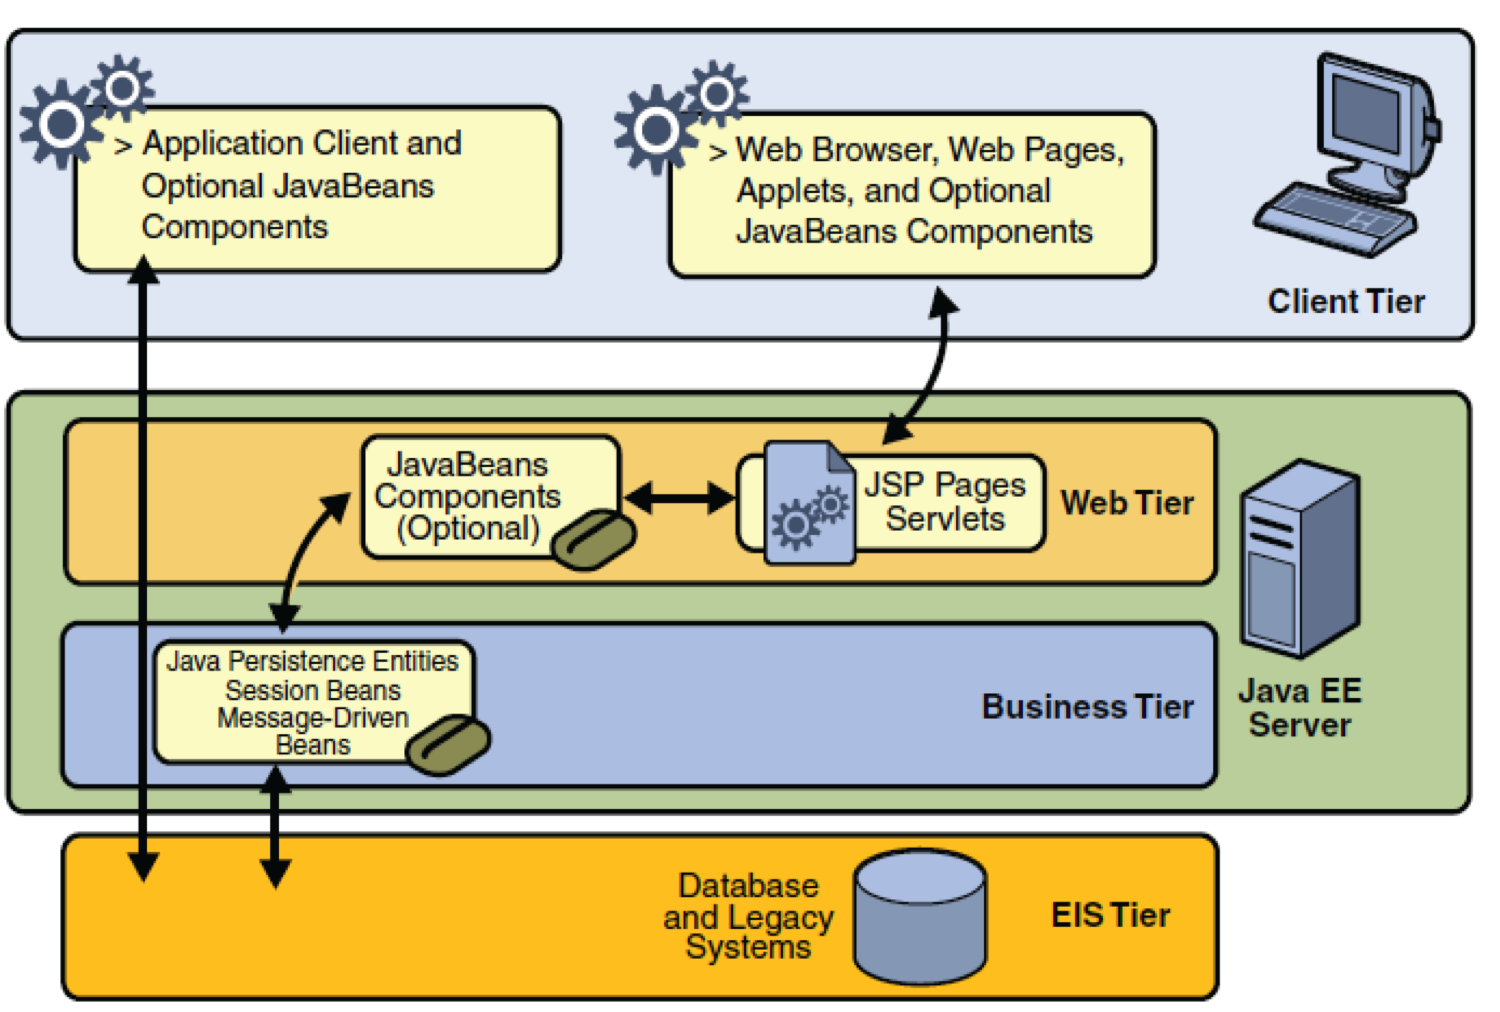
\includegraphics[width=0.7\textwidth]{fig05.png}
\end{figure}
\end{frame}

\begin{frame}
\frametitle{Java EE组件} 
\begin{itemize}
\item Application Client Component 
\item Applet Component
\item Web Component
  \begin{itemize}
  \item Servlet 
  \item JSP
  \end{itemize}
\item EJB Component
  \begin{itemize}
  \item Session Bean
  \item Entity Bean
  \item Message Driven Bean
  \end{itemize}
\end{itemize}
\end{frame}

\begin{frame}
\frametitle{客户端组件} 
\begin{itemize}
\item 客户端组件即JavaBean类,基于Java SE平台,运行在客户端容器内,有独立的JVM空间。
\item 客户端组件一般用富客户端图形界面显示,图形框架用Swing开发,可以远程调用Web组件和EJB组件。
\end{itemize}
\end{frame}

\begin{frame}
\frametitle{Applet组件} 
\begin{itemize}
\item Applet组件采用Java Applet框架技术开发,运行在Applet容器,即客户端Web浏览器,需要有Java SE的插件支持。
\item 目前客户端JavaBean组件和Applet组件已经逐渐被RIA(富互联网应用)技术取代,不推荐在企业级应用中使用客户端组件和Applet组件。
\end{itemize}
\end{frame}

\begin{frame}
\frametitle{Web组件} 
\begin{itemize}
\item Web组件运行在服务器端的Web容器内,能接收HTTP请求并进行处理,产生动态Web响应。
\item Web组件近十几年的互联网应用中得到广泛应用,一度成为Java EE的核心。
\item Java EE规定了两种类型的Web组件:Servlet组件和JSP组件。
\item 近年来,随着开发人员发现Web组件开发过于繁琐和细化,在Web组件基础上发布了各种用于简化Web组件开发的框架和技术,其中最著名的就是Struts框架,另外还有Spring Web MVC、JSF等,都是对标准Web组件的扩展和更新。
\end{itemize}
\end{frame}

\begin{frame}
\frametitle{EJB组件} 
\begin{itemize}
\item EJB组件运行在符合Java EE的应用服务器内,驻留在服务器端。Java EE的其他组件,包括EJB组件通过RMI/IIOP协议与EJB容器通信,远处调用EJB的功能方法,进而完成业务处理。
\item Java EE 5.0之前,EJB性能差,饱受诟病。Rod Johnson特别针对EJB的缺点,开发了轻量级的企业组件管理技术Spring,可以使用普通的JavaBean组件完全取代EJB组件。
\item Java EE 5.0之后,Sun公司全面引入Spring框架思想和Java SE 5.0的注释编程技术,推出了EJB 3.0组件规范。从而确立了EJB在大型企业软件项目开发中的地位。
\end{itemize}
\end{frame}

\section{Java EE服务API}

\begin{frame}
\frametitle{Java EE服务API} 

Java EE提供了标准化的服务接口API来统一各种外部资源的访问和控制。
\begin{figure}
\centering
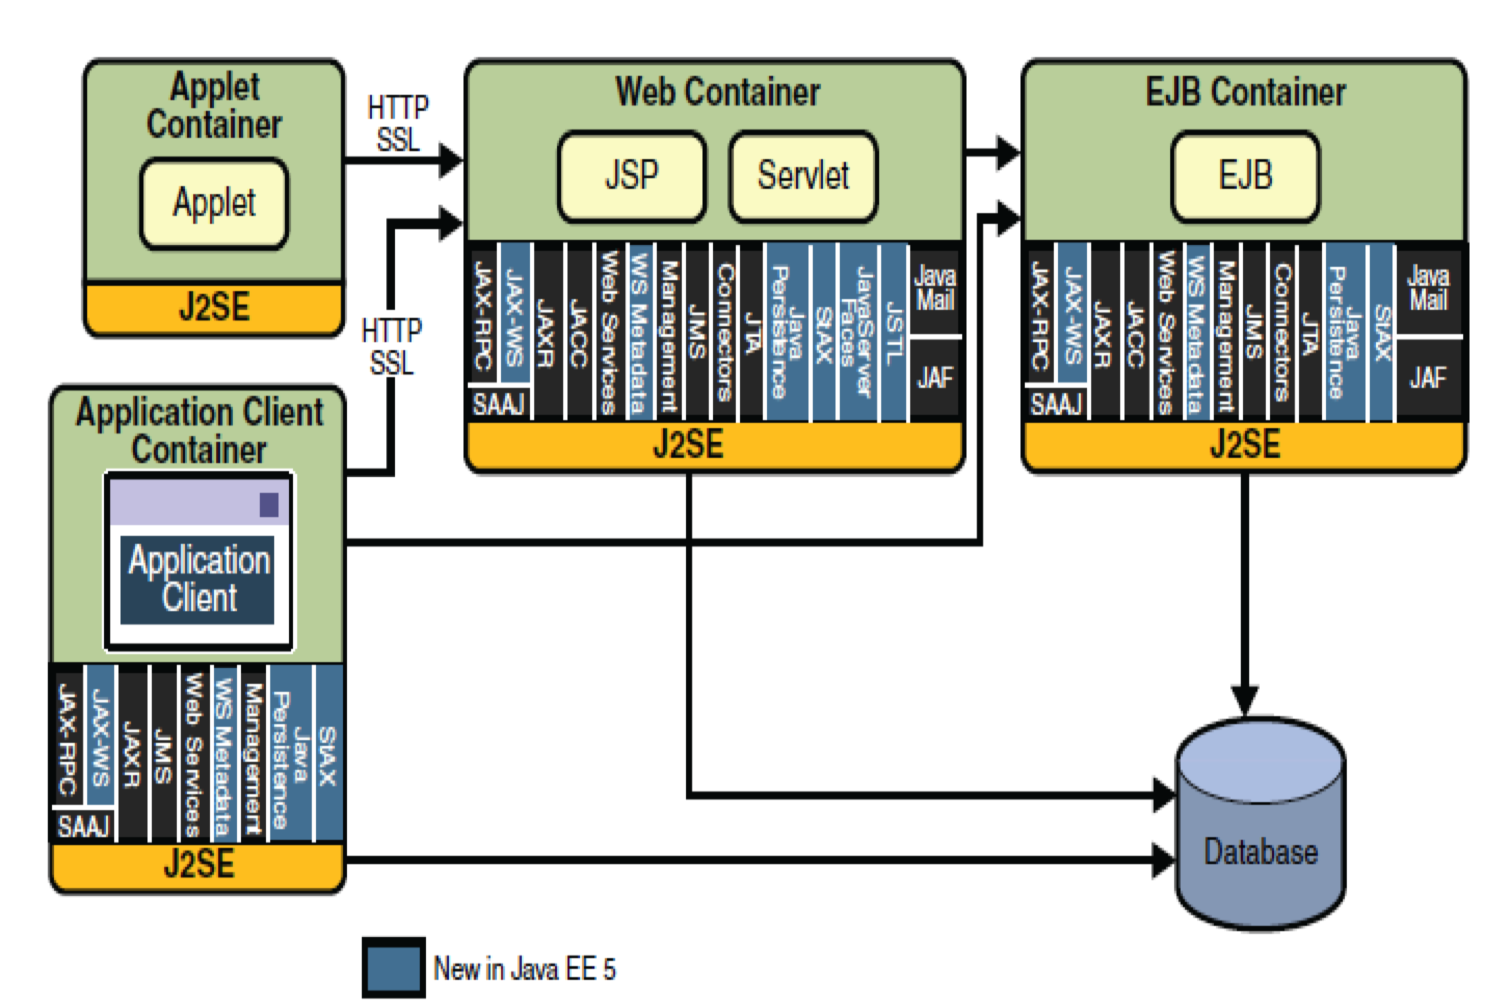
\includegraphics[width=0.85\textwidth]{fig06.png}
\end{figure} 
\end{frame}

\begin{frame}
\frametitle{Java EE服务API} 

\begin{itemize}
\item 数据库连接服务 API-JDBC
\item 消息服务连接服务 API-JMS
\item 数据持久化服务 API-JPA
\item 命名和目录服务 API-JNDI
\item 安全性和授权服务API-JAAS
\item 电子邮件服务 API-JavaMail
\item 事务服务 API-JTA
\item XML处理服务 API-JAXP
\item XML Web服务 API-JAX-WS
\item XML绑定服务 API-JAXB
\item 带附件的SOAP服务 API-SAAJ
\item XML Web服务注册 API-JAXR
\item 与其他遗留系统交互服务 API-J2EE Connector Architecture
\end{itemize}
\end{frame}

\section{组件间通信协议}
\begin{frame}
\frametitle{组件间通信协议} 

{\hei 各种Java EE组件运行在Java EE容器内,组件之间不允许直接取得对象引用和直接调用,只能使用规定的通信协议与组件所在的容器进行通信并请求目标组件。}

Java EE针对不同的容器指定了不同的通信协议。

\begin{figure}
\centering
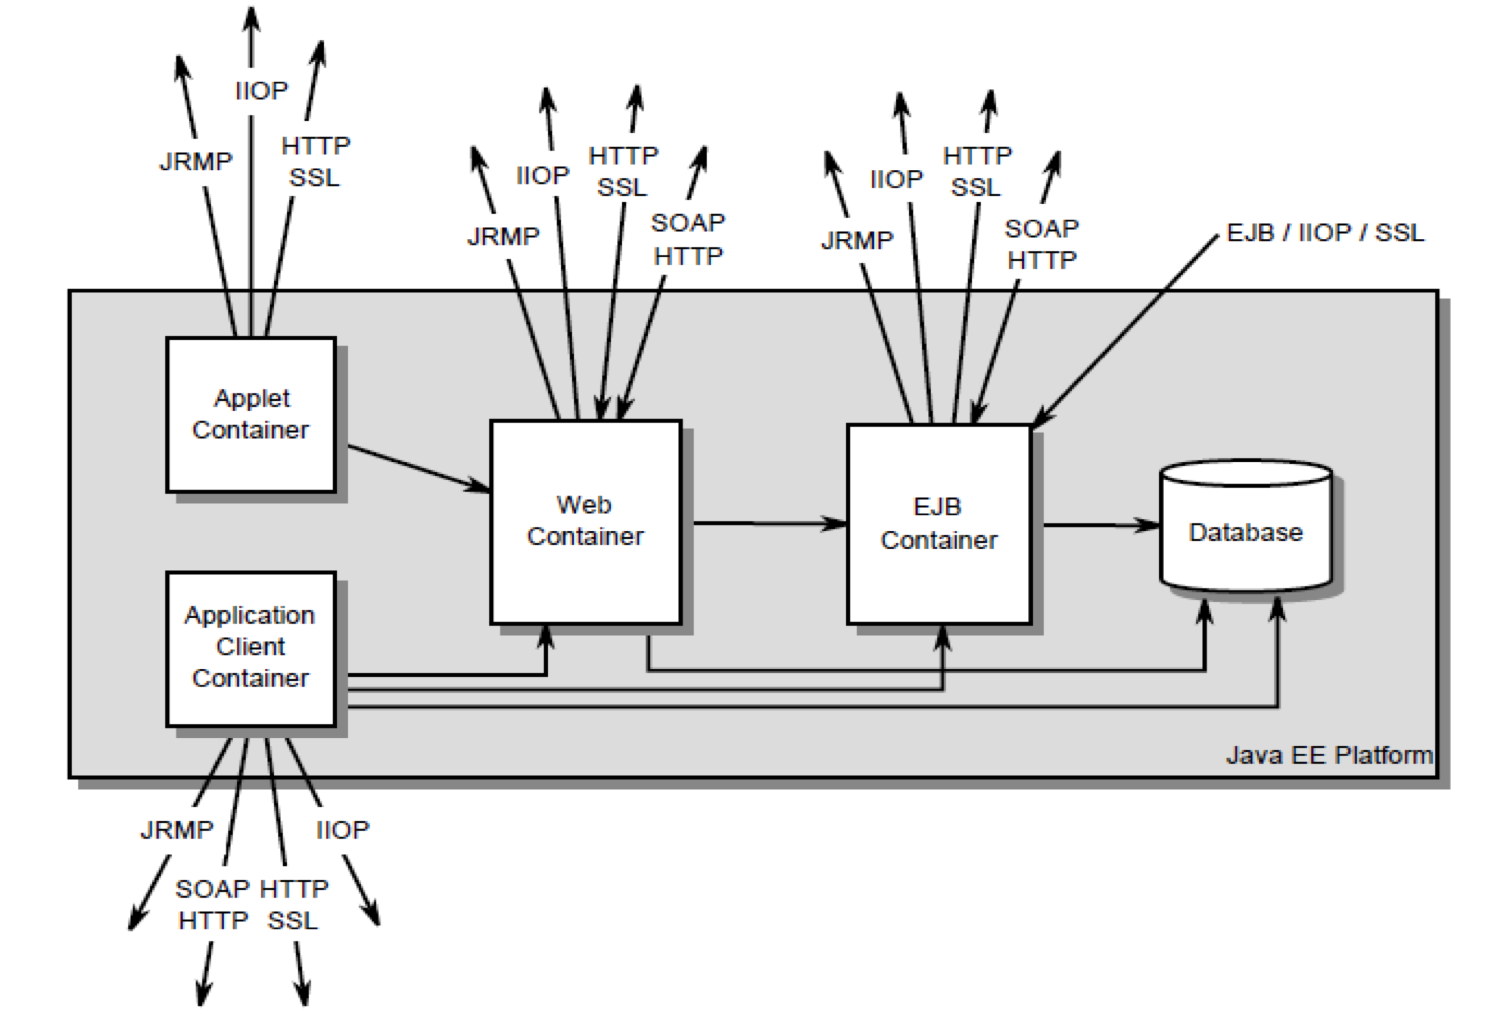
\includegraphics[width=0.75\textwidth]{fig07.png}
\end{figure} 
\end{frame}

\begin{frame}
\frametitle{HTTP and HTTPS} 
\kai
\wxd{HTTP} 

Java EE规范继续使用HTTP作为与Web容器通信的标准协议,延续了Web应用的标准化,使访问静态HTML页面和访问Java EE Web组件Servlet和JSB都使用相同的HTTP协议。

\wxd{HTTPS} 

... 
\end{frame}

\begin{frame}
\frametitle{RMI and RMI-IIOP} 
\kai
\wxd{RMI}

RMI (Remote Method Invocation),远程方法调用大大增强了Java开发分布式应用的能力,可以被认为是远程过程调用的Java版本。Java EE的EJB容器使用RMI协议进行通信。

\wxd{RMI-IIOP}

RMI-IIOP (Java Romote Method Invocation Over the Internet Inter-ORB Portocol)是RMI功能扩展版本,增加了如分布式垃圾收集和可下载类文件等,目前Java EE应用中与EJB容器和组件通信都是用RIM-IIOP。
\end{frame}

\begin{frame}
\frametitle{SOAP} 
\kai
\wxd{SOAP}

SOAP (Simple Object Access Protocol)是一种标准化的通信规范,主要用于与Web Services交互调用。SOAP以XML格式交换数据,使其与编程语言、平台和硬件无关。SOAP 1.2是业界共同的标准,属于第二代的XML协定(第一代主要为XML-RPC以及WDDX技术)。
\end{frame}

\section{Java EE的角色}

\begin{frame}
\frametitle{Java EE的角色} 
\begin{itemize}[<+-| alert@+>]
\item Java EE Product Provider\\
\only<1>{Sun GlassFish, Oracle BEA WebLogic, IBM WebSphere, JBOSS, Apache Tomcat}

\item Tool Provider\\
\only<2>{Sun NetBean, Eclipse Eclipse, Oracle JDevelpoer}

\item Application Component Provider\\

\item Application Assembler\\
\only<4>{Component, JAR, WAR \ding{223} Java EE EAR}

\item Deployer and System Administrator\\
\only<5>{
\ding{182} Deploy EAR files in the Java EE Server.\\
\ding{183} According to environment, modify and deploy configuration files, then manage Java EE system.\\
\ding{184} Varify the conformance from structure of EAR files to Java EE standards.}
\end{itemize}

某一角色的输出一般都是另一角色的输入。

\end{frame}
%%%%%%%%%%%%%%%%%%%%%%%%%%
\begin{frame}
\frametitle{} 

\end{frame}
%%%%%%%%%%%%%%%%%%%%%%%%%%
\begin{frame}
\frametitle{本章习题}
\begin{enumerate}
\item 简述Java EE的组件和功能。
\item 简述Java EE的容器类型和功能。
\item 理解当今软件开发的主要特点。
\end{enumerate}
\end{frame}

%%%%%%%%%%%%%%%%%%%%%%%%%%%%%%%%%%%%%%%%%%%%%%%%%%%%%%%%%%%%%%%%%%%%%%%%%%%%%%% 
\begin{frame}
\centering
{\Huge \textcolor{blue}{THE END}} \\
\vspace{5mm}
{\Large wangxiaodong@ouc.edu.cn} \\
\end{frame}
%%%%%%%%%%%%%%%%%%%%%%%%%%%%%%%%%%%%%%%%%%%%%%%%%%%%%%%%%%%%%%%%%%%%%%%%%%%%%%%
\end{document}
